\documentclass[12pt]{beamer}
\usepackage[utf8]{inputenc}
\usepackage[T1,T2A]{fontenc}
\usepackage[russian]{babel}
\usepackage{color}
\usepackage{listings}
\usepackage{calc}
\usepackage{graphicx}
\usepackage{epstopdf}
\usepackage{hyperref}
\usepackage{csquotes}
\usepackage{upquote}
%\usetheme{hohenheim}
\usetheme{Singapore} % Copenhagen, metropolis
%\usepackage[mono,varqu]{zi4}
\usepackage[defaultsans]{droidsans}
\usepackage[defaultmono]{droidmono}
\makeatletter
\input droid/t1fdm.fd
\makeatother
\lstset{
    language=Haskell,
    inputencoding=utf8,
    extendedchars=true,
    breaklines=true,
    escapeinside=!!,
    tabsize=4,
    breakatwhitespace=true,
    keepspaces=true
}
\lstset{
    literate={а}{{\selectfont\char224}}1
    {б}{{\selectfont\char225}}1
    {в}{{\selectfont\char226}}1
    {г}{{\selectfont\char227}}1
    {д}{{\selectfont\char228}}1
    {е}{{\selectfont\char229}}1
    {ё}{{\"e}}1
    {ж}{{\selectfont\char230}}1
    {з}{{\selectfont\char231}}1
    {и}{{\selectfont\char232}}1
    {й}{{\selectfont\char233}}1
    {к}{{\selectfont\char234}}1
    {л}{{\selectfont\char235}}1
    {м}{{\selectfont\char236}}1
    {н}{{\selectfont\char237}}1
    {о}{{\selectfont\char238}}1
    {п}{{\selectfont\char239}}1
    {р}{{\selectfont\char240}}1
    {с}{{\selectfont\char241}}1
    {т}{{\selectfont\char242}}1
    {у}{{\selectfont\char243}}1
    {ф}{{\selectfont\char244}}1
    {х}{{\selectfont\char245}}1
    {ц}{{\selectfont\char246}}1
    {ч}{{\selectfont\char247}}1
    {ш}{{\selectfont\char248}}1
    {щ}{{\selectfont\char249}}1
    {ъ}{{\selectfont\char250}}1
    {ы}{{\selectfont\char251}}1
    {ь}{{\selectfont\char252}}1
    {э}{{\selectfont\char253}}1
    {ю}{{\selectfont\char254}}1
    {я}{{\selectfont\char255}}1
    {А}{{\selectfont\char192}}1
    {Б}{{\selectfont\char193}}1
    {В}{{\selectfont\char194}}1
    {Г}{{\selectfont\char195}}1
    {Д}{{\selectfont\char196}}1
    {Е}{{\selectfont\char197}}1
    {Ё}{{\"E}}1
    {Ж}{{\selectfont\char198}}1
    {З}{{\selectfont\char199}}1
    {И}{{\selectfont\char200}}1
    {Й}{{\selectfont\char201}}1
    {К}{{\selectfont\char202}}1
    {Л}{{\selectfont\char203}}1
    {М}{{\selectfont\char204}}1
    {Н}{{\selectfont\char205}}1
    {О}{{\selectfont\char206}}1
    {П}{{\selectfont\char207}}1
    {Р}{{\selectfont\char208}}1
    {С}{{\selectfont\char209}}1
    {Т}{{\selectfont\char210}}1
    {У}{{\selectfont\char211}}1
    {Ф}{{\selectfont\char212}}1
    {Х}{{\selectfont\char213}}1
    {Ц}{{\selectfont\char214}}1
    {Ч}{{\selectfont\char215}}1
    {Ш}{{\selectfont\char216}}1
    {Щ}{{\selectfont\char217}}1
    {Ъ}{{\selectfont\char218}}1
    {Ы}{{\selectfont\char219}}1
    {Ь}{{\selectfont\char220}}1
    {Э}{{\selectfont\char221}}1
    {Ю}{{\selectfont\char222}}1
    {Я}{{\selectfont\char223}}1
}
\lstset{
    basicstyle=\ttfamily\footnotesize,
    commentstyle=\color{green}\itshape,
    % keywordstyle=\color{blue} % TODO https://tex.stackexchange.com/questions/415777/avoid-highlighting-keywords-following-certain-words-in-listings
}

\begin{document}
	\author{Алексей Романов}
	\title{Функциональное программирование на Haskell}
	\subtitle{Лекция 1: введение}
	%\logo{}
	%\institute{}
	%\date{}
	\subject{Функциональное программирование на Haskell}
	%\setbeamercovered{transparent}
	%\setbeamertemplate{navigation symbols}{}
	\begin{frame}[plain]
	\maketitle
\end{frame}

\begin{frame}
\frametitle{Организация курса}
\begin{itemize}
    \item 8 лекций
    \item 4 лабораторных
    \item Итоговый проект
\end{itemize}
\end{frame}

\begin{frame}
\frametitle{Парадигмы программирования}
Что такое парадигма? \\
\pause
\hspace*{20pt} Совокупность идей и понятий, определяющих стиль написания компьютерных программ. \\
\pause
Основные парадигмы: \\
\pause
\begin{itemize}
    \item Структурное программирование
    \item Процедурное программирование
    \item \textbf{Функциональное программирование}
    \item Логическое программирование
    \item Объектно-ориентированное программирование
\end{itemize}
\pause
В парадигме важно не только то, что используется, но то, использование чего не допускается или минимизируется.
\pause
Например, \lstinline!goto! в структурном программировании, глобальные переменные в ООП.
\end{frame}

\begin{frame}
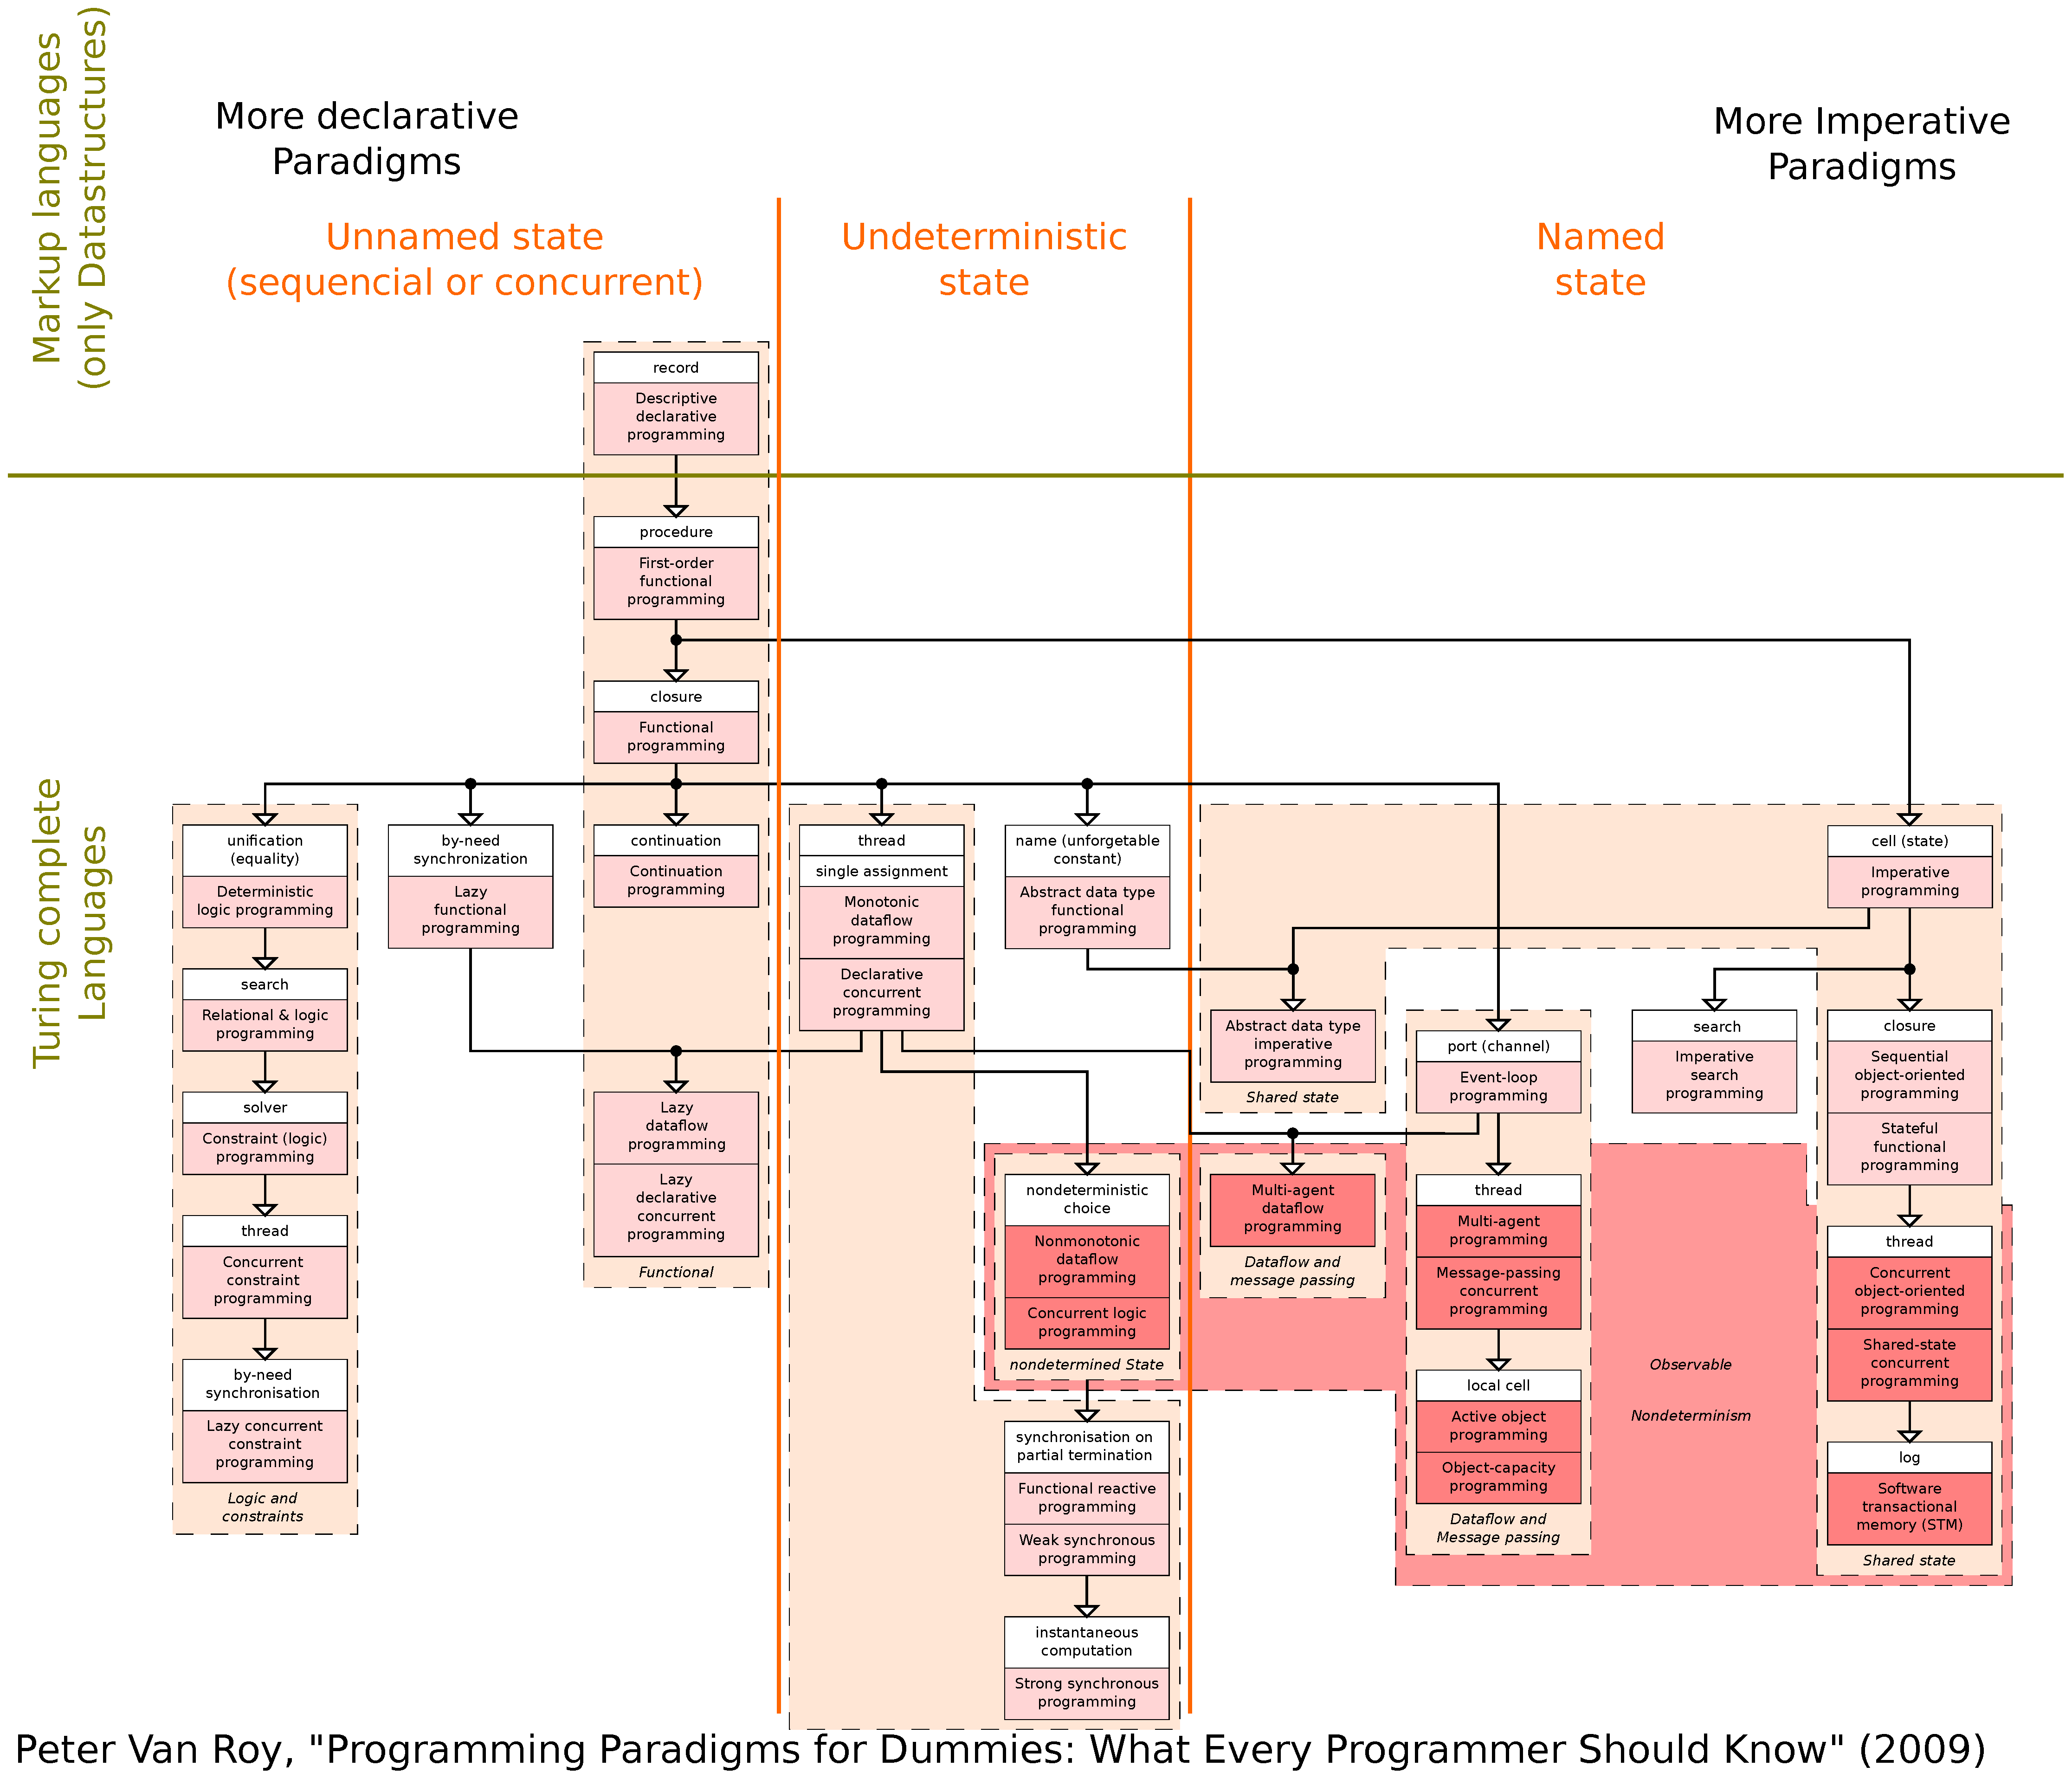
\includegraphics[scale=0.13]{lecture1_programming_paradigms.eps}
\end{frame}

\begin{frame}
\frametitle{Функциональное программирование}
\begin{itemize}
    \item Значения лучше переменных.
    \begin{itemize}
        \item Переменная даёт имя значению или функции, а не адресу в памяти.
        \item Переменные неизменяемы.
        \item Типы данных неизменяемы.
    \end{itemize}
    \item Выражения лучше инструкций.
    \begin{itemize}
        \item Аналоги \lstinline|if|, \lstinline|try-catch| и т.д. -- выражения.
    \end{itemize}
    \item Функции как в математике (следующий слайд)
\end{itemize}
\end{frame}


\begin{frame}
\frametitle{Функциональное программирование}
\begin{itemize}
    \item Функции как в математике\pause
    \begin{itemize}
        \item Чистые функции: аргументу соответствует результат, а всё прочее от лукавого.
        \begin{itemize}
            \item Нет побочных эффектов (ввода-вывода, обращения к внешней памяти, не связанной с аргументом, и т.д.)
            \item При одинаковых аргументах результаты такой функции одинаковы
        \end{itemize}
        \item Функции являются значениями (функции первого класса)
        \item Функции часто принимают и возвращают функции (функции высших порядков)
    \end{itemize}
    \pause
    \item Опора на математические теории: лямбда-исчисление, теория типов, теория категорий
\end{itemize}
\end{frame}

\begin{frame}
\frametitle{Языки ФП}
\begin{itemize}
    \item семейство Lisp: первый ФП-язык и один из первых языков высокого уровня вообще
    \item Erlang и Elixir: упор на многозадачность (модель акторов), надёжность
    \item Scala, Kotlin, F\#: гибриды с ООП для JVM и для CLR
    \item Purescript, Elm, Ur/Web: для веба
    \item Семейство ML: OCaml, SML, F\#
    \pause
    \item \textbf{Haskell:}
    \begin{itemize}
        \item Чисто функциональный
        \pause
        \item Строго статически типизированный (с очень мощной и выразительной системой типов)
        \pause
        \item Ленивый
    \end{itemize}
\end{itemize}
\end{frame}

\begin{frame}[fragile]
\frametitle{Язык Haskell: начало}
\begin{itemize}
    \item Установите Haskell Platform (\url{https://www.haskell.org/platform/})
    \item Запустите WinGHCi (или просто GHCi)
    \item Это оболочка или REPL (Read-Eval-Print loop) для Haskell
    \begin{itemize}
        \item Read: Вы вводите выражения (и команды GHCi)
        \item Eval: GHCi вычисляет результат
        \item Print: и выводит его на экран
    \end{itemize}
    \item Пример:
\begin{lstlisting}[breaklines]
GHCi, version 8.2.2: http://www.haskell.org/ghc/  :? for help
Prelude> 2 + 2
4
Prelude> :t True -- команда GHCi
True :: Bool
\end{lstlisting}
\end{itemize}
\end{frame}

\begingroup
\footnotesize
\begin{frame}[fragile]
\frametitle{Язык Haskell: начало}
\begin{itemize}
    \item \lstinline|2 + 2|, \lstinline|True|: выражения
    \item \lstinline|4|, \lstinline|True|: значения
    \item \lstinline|Bool|: тип
    \pause
    \item Значение: \enquote{вычисленное до конца} выражение
    \item Тип (статический): множество значений и выражений, построенное по определённым законам таким образом, что компилятор может определить типы и проверить отсутствие ошибок в них без запуска программы.
    \item От типа зависит то, какие операции допустимы:
\begin{lstlisting}[basicstyle=\ttfamily\scriptsize]
Prelude> True + False

<interactive>:12:1: error:
No instance for (Num Bool) arising from a use of '+'
In the expression: True + False
In an equation for 'it': it = True + False
\end{lstlisting}
\end{itemize}
\end{frame}
\endgroup

\begin{frame}[fragile]
\frametitle{Вызов функций}
\begin{itemize}
    \item Вызов (применение) функции пишется без скобок: \lstinline|f x|, \lstinline|foo x y|. 
    \item Скобки используются, когда аргументы -- сложные выражения, а не переменные: \lstinline|f (g x)| (и внутри сложных выражений вообще).
    \item Бинарные операторы (как \lstinline|+|) это просто функции.
    \begin{itemize}
        \item Можно писать их префиксно, заключив в скобки: \lstinline[breaklines=false]|(+) 2 2|
        \item А любую функцию двух аргументов можно писать инфиксно, заключив в обратный апостроф: \lstinline|4 `div` 2|
    \end{itemize}
    \item Названия переменных и функций начинаются со строчной буквы
        \begin{itemize}
            \item или состоят целиком из спец. символов.
        \end{itemize}
\end{itemize}
\end{frame}

\begin{frame}[fragile]
\frametitle{Определение функций и переменных}
\begin{itemize}
    \item Определение функции выглядит так же как вызов:
\begin{lstlisting}[breaklines]
название параметр1 параметр2 = значение
название = значение -- переменная
\end{lstlisting}
    \item Тело функции это не блок, а одно выражение (но сколь угодно сложное).
    \item В GHCi перед определением нужен \lstinline|let|, в отличие от кода в файлах: 
\begin{lstlisting}
Prelude> let x = sin pi
Prelude> x !\pause!
1.2246063538223773e-16
Prelude> let square x = x * x
Prelude> square 2
4
\end{lstlisting}
\end{itemize}
\end{frame}

\begingroup
\small

\begin{frame}[fragile]
\frametitle{Базовые типы}
\begin{itemize}
    \item Названия типов всегда начинаются с заглавной буквы (или состоят целиком из спец. символов).
    \item \lstinline|Bool|: логические значения \lstinline|True| и \lstinline|False|.
    \item Целые числа:
    \begin{itemize}
        \item \footnotesize \lstinline|Integer|: неограниченные (кроме размера памяти);
        \item \footnotesize \lstinline|Int|: машинные\footnote{по cтандарту минимум 30 бит, но в GHC это 32 или 64 бита}, \lstinline|Word|: машинные без знака;
        \item \footnotesize \lstinline|Data.{Int.Int/Word.Word}{8/16/32/64}|: фиксированного размера в битах, со знаком и без.
    \end{itemize}
    \item \lstinline|Float| и \lstinline|Double|: 32- и 64-битные числа с плавающей точкой.
    \item \lstinline|Character|: символы Unicode.
    \item \lstinline|()|: Unit (единичный тип), единственное значение \lstinline|()|.
\end{itemize}
\end{frame}

\endgroup

\begin{frame}[fragile]
\frametitle{Тип функций и сигнатуры}
\begin{itemize}
    \item Типы функций записываются через \lstinline|->|. Например, \lstinline|Int -> Char| это тип функции из \lstinline|Int| в \lstinline|Char|.
    
    \item Для нескольких аргументов это выглядит как \pause\lstinline|Bool -> Bool -> Bool|.
    
    \item \lstinline|::| читается как \enquote{имеет тип}; запись \lstinline|выражение :: тип| называется \enquote{сигнатурой типа}.
    
    \item При объявлении экспортируемой функции или переменной  сигнатура обычно указывается явно:
\begin{lstlisting}
foo :: Int -> Char
foo x = ...
\end{lstlisting}
    \item Компилятор обычно выведет типы и без этого, но явное указание защищает от \emph{непреднамеренного} изменения.
\end{itemize}
\end{frame}

\begin{frame}[fragile]
\frametitle{Арифметика}
\begin{itemize}
    \item Это упрощённая версия, так как настоящее объяснение требует понятия класса типов, которое будет введено позже. 
    \item Например, \lstinline|:type 1| или \lstinline|:type (+)| дадут тип, который понимать пока не требуется. 
    \item То же относится к ошибкам вроде \lstinline[breaklines=false]|No instance for (Num Bool) arising from a use of '+'| на более раннем слайде.
    \item Пока достаточно понимать, что есть понятие \enquote{числового типа}, которые делятся на целочисленные (\lstinline|Int|, \lstinline|Integer|) и дробные (\lstinline|Float|, \lstinline|Double|).
\end{itemize}
\end{frame}

\begin{frame}[fragile]
\frametitle{Числовые литералы}
\begin{itemize}
    \item Числовые литералы выглядят, как в других языках: \lstinline|0|, \lstinline|1.5|, \lstinline|1.2E-1|, \lstinline|0xDEADBEEF|. 
    \item Целочисленные литералы могут иметь любой числовой тип, а дробные любой дробный.
    \item Но это относится \emph{только} к литералам. Неявного приведения (например, \lstinline|Int| в \lstinline|Double|) в Haskell \emph{нет}. 
\end{itemize}
\end{frame}

\begin{frame}[fragile]
\frametitle{Приведение числовых типов}
\begin{itemize}
    \item Используйте \lstinline|fromIntegral| для приведения из любого целочисленного типа в любой числовой. Тип-цель можно указать явно:
\begin{lstlisting}
Prelude> let {x :: Integer; x = 2}
Prelude> x :: Double
<interactive>:22:1: error:
Couldn't match expected type 'Double' with actual type 'Integer' ...
Prelude> fromIntegral x :: Double
2.0
\end{lstlisting}    
    \item Или не указывать, если компилятор может его вывести из контекста:
\begin{lstlisting}
Prelude> :t fromIntegral 2 / (4 :: Double)
fromIntegral 2 / (4 :: Double) :: Double
\end{lstlisting}    
\end{itemize}
\end{frame}

\begin{frame}[fragile]
\frametitle{Приведение числовых типов}
\begin{itemize}
    \item \lstinline|toInteger| переводит любой целочисленный тип в \lstinline|Integer|, \lstinline|fromInteger| из \lstinline|Integer| в любой целочисленный.
    \begin{itemize}
        \item Если аргумент \lstinline|fromInteger| слишком велик для типа цели, берётся его значение по модулю:
        \begin{lstlisting}
Prelude> fromInteger (2^64) :: Int
0
\end{lstlisting}
    \end{itemize}
    \item \lstinline|toRational| и \lstinline|fromRational| -- аналогично для \lstinline|Rational| и дробных типов.
    \item \lstinline|ceiling|, \lstinline|floor|, \lstinline|truncate| и \lstinline|round| из дробных типов в целочисленные (по названиям должно быть понятно, как именно).
\end{itemize}
\end{frame}

\begin{frame}[fragile]
\frametitle{Арифметические операции}
\begin{itemize}
    \item Операции \lstinline|+|, \lstinline|-|, \lstinline|*| -- как в других языках, только аргументы обязательно имеют одинаковый тип.
    \item Унарный минус -- единственный унарный оператор.
    \item \lstinline|/| -- деление \emph{дробных} чисел, \lstinline|div| -- целочисленное, \lstinline|mod| -- остаток (есть ещё \lstinline|quot| и \lstinline|rem|, они отличаются поведением на отрицательных числах).
    \begin{itemize}
        \item Использование \lstinline|/| для целых чисел даст ошибку \lstinline|No instance... arising from a use of '/'|. Нужно сначала использовать \lstinline|fromIntegral|.
    \end{itemize}        
    \item \lstinline|^| -- возведение любого числа в целую неотрицательную степень, \lstinline|^^| -- дробного в любую целую, \lstinline|**| -- дробного в степень того же типа.
\end{itemize}
\end{frame}

\begin{frame}[fragile]
\frametitle{Операции сравнения и\\логические операции}
\begin{itemize}
    \item Большинство операций сравнения выглядят как обычно: \lstinline|==|, \lstinline|>|, \lstinline|<|, \lstinline|>=|.
    \item Но $\leq$ обозначается как \lstinline|=<|, а не \lstinline|<=|.
    \item А $\neq$ как \lstinline|/=|.
    \item Функция \lstinline|compare| возвращает \lstinline|Ordering|: тип с тремя значениями \lstinline|LT|, \lstinline|EQ| и \lstinline|GT|.
    \item Функции \lstinline|min| и \lstinline|max|.
    \item[]
    \item \enquote{и} это \lstinline|&&|, а \enquote{или} -- \lstinline!||!, как обычно. 
    \item \enquote{не} -- \lstinline|not|.
\end{itemize}
\end{frame}

\begin{frame}[fragile]
\frametitle{Существенные отступы (двухмерный синтаксис)}
\begin{itemize}
    \item TODO
\end{itemize}
\end{frame}

\begin{frame}[fragile]
\frametitle{Условные выражения}
\begin{itemize}
    \item В любом языке должна быть возможность выдать результат в зависимости от какого-то условия.
    \item Первый способ сделать это в Haskell: выражения \lstinline|if| и \lstinline|case|.
    \item Синтаксис \lstinline|if|: \lstinline|if условие then выражение1 else выражение2|. Поскольку это выражение, то \lstinline|else| обязательно! \lstinline|условие| имеет тип \lstinline|Bool|, \lstinline|выражение1| и \lstinline|выражение2| -- любой одинаковый тип, который будет и типом всего  \lstinline|if ... then ... else ...|. Это ближе к \lstinline|?:|, чем к \lstinline|if| в C-подобных языках.
    \item Многострочно пишется так:
\begin{lstlisting}
if условие 
    then выражение1 
    else выражение2
\end{lstlisting}
\end{itemize}
\end{frame}

\begingroup
\footnotesize
\begin{frame}[fragile]
\frametitle{Сопоставление с образцом}
\begin{itemize}
    \item Синтаксис \lstinline|case|: \\
\begin{lstlisting}
case выражение of 
    образец1 -> выражение1 
    образец2 -> выражение2
\end{lstlisting}
    \item Его смысл: вычислить значение \lstinline|выражение| и сопоставить с каждым образцом по очереди. Если первым подошёл \lstinline|образецN|, вернуть значение \lstinline|выражениеN|.
    \item Если ни один образец не подошёл, то вычисление \lstinline|case| выкидывает ошибку.
    \item В первом приближении, образец это \enquote{форма для значения}, которая может содержать неопределённые переменные (они получат значение при удачном сопоставлении). 
    \item Образцы похожи на выражения, но ими не являются: это новая синтаксическая категория!
\end{itemize}
\end{frame}
\endgroup

\begin{frame}[fragile]
\frametitle{Образцы для известных нам типов}
\begin{itemize}
%    \item 
%    \begin{itemize}
    \item \lstinline|True| и \lstinline|False| -- образцы для \lstinline|Bool|. Они подходят, только если значение совпадает с ними. 
    \item Аналогично \lstinline|LT|, \lstinline|EQ| и \lstinline|GT| для \lstinline|Ordering|, а числовые литералы для числовых типов.
    \item Переменная -- образец для любого типа. Она подходит для любого значения, и получает это значение при сопоставлении.
\item \lstinline|_| тоже образец для любого типа, который подходит для всех значений, но ничего не связывает. Можно читать как \enquote{значение не важно}.
%    \end{itemize}
\end{itemize}
\end{frame}

\begin{frame}[fragile]
\frametitle{Связь \lstinline[basicstyle=\ttfamily]|case| и \lstinline[basicstyle=\ttfamily]|if|}
\begin{itemize}
    \item Пример:
\begin{lstlisting}
if условие 
    then выражение1 
    else выражение2
\end{lstlisting}
это ровно то же самое, что
\begin{lstlisting}
case условие of
    True -> выражение1 
    False -> выражение2
\end{lstlisting}
    На самом деле, при компиляции Haskell это преобразование действительно делается, чтобы не дублировать правила оптимизации.
\end{itemize}
\end{frame}


\begin{frame}[fragile]
\frametitle{Охраняющие условия}
\begin{itemize}
    \item У каждого образца могут быть дополнительные условия, которые могут содержать переменные из образца: 
\begin{lstlisting}
образец
    | условие1 -> выражение1 
    | условие2 -> выражение2
\end{lstlisting}
В этом случае при удачном сопоставлении проверяется по очереди каждое условие. Если ни одно из них не выполнено, сопоставление переходит к следующему образцу.
\end{itemize}
\end{frame}

\begin{frame}[fragile]
\frametitle{Определение функций по случаям}
\begin{itemize}
    \item TODO
\end{itemize}
\end{frame}

\begin{frame}[fragile]
\frametitle{Локальные переменные}
\begin{itemize}
    \item TODO
\end{itemize}
\end{frame}

\end{document}